% Options for packages loaded elsewhere
\PassOptionsToPackage{unicode}{hyperref}
\PassOptionsToPackage{hyphens}{url}
%
\documentclass[
]{article}
\usepackage{amsmath,amssymb}
\usepackage{iftex}
\ifPDFTeX
  \usepackage[T1]{fontenc}
  \usepackage[utf8]{inputenc}
  \usepackage{textcomp} % provide euro and other symbols
\else % if luatex or xetex
  \usepackage{unicode-math} % this also loads fontspec
  \defaultfontfeatures{Scale=MatchLowercase}
  \defaultfontfeatures[\rmfamily]{Ligatures=TeX,Scale=1}
\fi
\usepackage{lmodern}
\ifPDFTeX\else
  % xetex/luatex font selection
\fi
% Use upquote if available, for straight quotes in verbatim environments
\IfFileExists{upquote.sty}{\usepackage{upquote}}{}
\IfFileExists{microtype.sty}{% use microtype if available
  \usepackage[]{microtype}
  \UseMicrotypeSet[protrusion]{basicmath} % disable protrusion for tt fonts
}{}
\makeatletter
\@ifundefined{KOMAClassName}{% if non-KOMA class
  \IfFileExists{parskip.sty}{%
    \usepackage{parskip}
  }{% else
    \setlength{\parindent}{0pt}
    \setlength{\parskip}{6pt plus 2pt minus 1pt}}
}{% if KOMA class
  \KOMAoptions{parskip=half}}
\makeatother
\usepackage{xcolor}
\usepackage[margin=2.54cm]{geometry}
\usepackage{color}
\usepackage{fancyvrb}
\newcommand{\VerbBar}{|}
\newcommand{\VERB}{\Verb[commandchars=\\\{\}]}
\DefineVerbatimEnvironment{Highlighting}{Verbatim}{commandchars=\\\{\}}
% Add ',fontsize=\small' for more characters per line
\usepackage{framed}
\definecolor{shadecolor}{RGB}{248,248,248}
\newenvironment{Shaded}{\begin{snugshade}}{\end{snugshade}}
\newcommand{\AlertTok}[1]{\textcolor[rgb]{0.94,0.16,0.16}{#1}}
\newcommand{\AnnotationTok}[1]{\textcolor[rgb]{0.56,0.35,0.01}{\textbf{\textit{#1}}}}
\newcommand{\AttributeTok}[1]{\textcolor[rgb]{0.13,0.29,0.53}{#1}}
\newcommand{\BaseNTok}[1]{\textcolor[rgb]{0.00,0.00,0.81}{#1}}
\newcommand{\BuiltInTok}[1]{#1}
\newcommand{\CharTok}[1]{\textcolor[rgb]{0.31,0.60,0.02}{#1}}
\newcommand{\CommentTok}[1]{\textcolor[rgb]{0.56,0.35,0.01}{\textit{#1}}}
\newcommand{\CommentVarTok}[1]{\textcolor[rgb]{0.56,0.35,0.01}{\textbf{\textit{#1}}}}
\newcommand{\ConstantTok}[1]{\textcolor[rgb]{0.56,0.35,0.01}{#1}}
\newcommand{\ControlFlowTok}[1]{\textcolor[rgb]{0.13,0.29,0.53}{\textbf{#1}}}
\newcommand{\DataTypeTok}[1]{\textcolor[rgb]{0.13,0.29,0.53}{#1}}
\newcommand{\DecValTok}[1]{\textcolor[rgb]{0.00,0.00,0.81}{#1}}
\newcommand{\DocumentationTok}[1]{\textcolor[rgb]{0.56,0.35,0.01}{\textbf{\textit{#1}}}}
\newcommand{\ErrorTok}[1]{\textcolor[rgb]{0.64,0.00,0.00}{\textbf{#1}}}
\newcommand{\ExtensionTok}[1]{#1}
\newcommand{\FloatTok}[1]{\textcolor[rgb]{0.00,0.00,0.81}{#1}}
\newcommand{\FunctionTok}[1]{\textcolor[rgb]{0.13,0.29,0.53}{\textbf{#1}}}
\newcommand{\ImportTok}[1]{#1}
\newcommand{\InformationTok}[1]{\textcolor[rgb]{0.56,0.35,0.01}{\textbf{\textit{#1}}}}
\newcommand{\KeywordTok}[1]{\textcolor[rgb]{0.13,0.29,0.53}{\textbf{#1}}}
\newcommand{\NormalTok}[1]{#1}
\newcommand{\OperatorTok}[1]{\textcolor[rgb]{0.81,0.36,0.00}{\textbf{#1}}}
\newcommand{\OtherTok}[1]{\textcolor[rgb]{0.56,0.35,0.01}{#1}}
\newcommand{\PreprocessorTok}[1]{\textcolor[rgb]{0.56,0.35,0.01}{\textit{#1}}}
\newcommand{\RegionMarkerTok}[1]{#1}
\newcommand{\SpecialCharTok}[1]{\textcolor[rgb]{0.81,0.36,0.00}{\textbf{#1}}}
\newcommand{\SpecialStringTok}[1]{\textcolor[rgb]{0.31,0.60,0.02}{#1}}
\newcommand{\StringTok}[1]{\textcolor[rgb]{0.31,0.60,0.02}{#1}}
\newcommand{\VariableTok}[1]{\textcolor[rgb]{0.00,0.00,0.00}{#1}}
\newcommand{\VerbatimStringTok}[1]{\textcolor[rgb]{0.31,0.60,0.02}{#1}}
\newcommand{\WarningTok}[1]{\textcolor[rgb]{0.56,0.35,0.01}{\textbf{\textit{#1}}}}
\usepackage{longtable,booktabs,array}
\usepackage{calc} % for calculating minipage widths
% Correct order of tables after \paragraph or \subparagraph
\usepackage{etoolbox}
\makeatletter
\patchcmd\longtable{\par}{\if@noskipsec\mbox{}\fi\par}{}{}
\makeatother
% Allow footnotes in longtable head/foot
\IfFileExists{footnotehyper.sty}{\usepackage{footnotehyper}}{\usepackage{footnote}}
\makesavenoteenv{longtable}
\usepackage{graphicx}
\makeatletter
\def\maxwidth{\ifdim\Gin@nat@width>\linewidth\linewidth\else\Gin@nat@width\fi}
\def\maxheight{\ifdim\Gin@nat@height>\textheight\textheight\else\Gin@nat@height\fi}
\makeatother
% Scale images if necessary, so that they will not overflow the page
% margins by default, and it is still possible to overwrite the defaults
% using explicit options in \includegraphics[width, height, ...]{}
\setkeys{Gin}{width=\maxwidth,height=\maxheight,keepaspectratio}
% Set default figure placement to htbp
\makeatletter
\def\fps@figure{htbp}
\makeatother
\setlength{\emergencystretch}{3em} % prevent overfull lines
\providecommand{\tightlist}{%
  \setlength{\itemsep}{0pt}\setlength{\parskip}{0pt}}
\setcounter{secnumdepth}{-\maxdimen} % remove section numbering
\ifLuaTeX
  \usepackage{selnolig}  % disable illegal ligatures
\fi
\IfFileExists{bookmark.sty}{\usepackage{bookmark}}{\usepackage{hyperref}}
\IfFileExists{xurl.sty}{\usepackage{xurl}}{} % add URL line breaks if available
\urlstyle{same}
\hypersetup{
  pdftitle={ENV 790.30 - Time Series Analysis for Energy Data \textbar{} Spring 2024},
  pdfauthor={Julia Kagiliery},
  hidelinks,
  pdfcreator={LaTeX via pandoc}}

\title{ENV 790.30 - Time Series Analysis for Energy Data \textbar{}
Spring 2024}
\usepackage{etoolbox}
\makeatletter
\providecommand{\subtitle}[1]{% add subtitle to \maketitle
  \apptocmd{\@title}{\par {\large #1 \par}}{}{}
}
\makeatother
\subtitle{Assignment 2 - Due date 02/25/24}
\author{Julia Kagiliery}
\date{}

\begin{document}
\maketitle

\hypertarget{submission-instructions}{%
\subsection{Submission Instructions}\label{submission-instructions}}

You should open the .rmd file corresponding to this assignment on
RStudio. The file is available on our class repository on Github.

Once you have the file open on your local machine the first thing you
will do is rename the file such that it includes your first and last
name (e.g., ``LuanaLima\_TSA\_A02\_Sp24.Rmd''). Then change ``Student
Name'' on line 4 with your name.

Then you will start working through the assignment by \textbf{creating
code and output} that answer each question. Be sure to use this
assignment document. Your report should contain the answer to each
question and any plots/tables you obtained (when applicable).

When you have completed the assignment, \textbf{Knit} the text and code
into a single PDF file. Submit this pdf using Sakai.

\hypertarget{r-packages}{%
\subsection{R packages}\label{r-packages}}

R packages needed for this assignment:``forecast'',``tseries'', and
``dplyr''. Install these packages, if you haven't done yet. Do not
forget to load them before running your script, since they are NOT
default packages.\textbackslash{}

\begin{Shaded}
\begin{Highlighting}[]
\CommentTok{\#Load/install required package here}
\FunctionTok{library}\NormalTok{(dplyr)}
\end{Highlighting}
\end{Shaded}

\begin{verbatim}
## 
## Attaching package: 'dplyr'
\end{verbatim}

\begin{verbatim}
## The following objects are masked from 'package:stats':
## 
##     filter, lag
\end{verbatim}

\begin{verbatim}
## The following objects are masked from 'package:base':
## 
##     intersect, setdiff, setequal, union
\end{verbatim}

\begin{Shaded}
\begin{Highlighting}[]
\FunctionTok{library}\NormalTok{(tseries)}
\end{Highlighting}
\end{Shaded}

\begin{verbatim}
## Registered S3 method overwritten by 'quantmod':
##   method            from
##   as.zoo.data.frame zoo
\end{verbatim}

\begin{Shaded}
\begin{Highlighting}[]
\FunctionTok{library}\NormalTok{(forecast) }
\FunctionTok{library}\NormalTok{(lubridate)}
\end{Highlighting}
\end{Shaded}

\begin{verbatim}
## 
## Attaching package: 'lubridate'
\end{verbatim}

\begin{verbatim}
## The following objects are masked from 'package:base':
## 
##     date, intersect, setdiff, union
\end{verbatim}

\begin{Shaded}
\begin{Highlighting}[]
\FunctionTok{library}\NormalTok{(ggplot2)}
\FunctionTok{library}\NormalTok{(tinytex)}
\end{Highlighting}
\end{Shaded}

\hypertarget{data-set-information}{%
\subsection{Data set information}\label{data-set-information}}

Consider the data provided in the spreadsheet
``Table\_10.1\_Renewable\_Energy\_Production\_and\_Consumption\_by\_Source.xlsx''
on our \textbf{Data} folder. The data comes from the US Energy
Information and Administration and corresponds to the December 2023
Monthly Energy Review. The spreadsheet is ready to be used. You will
also find a \(.csv\) version of the data
``Table\_10.1\_Renewable\_Energy\_Production\_and\_Consumption\_by\_Source-Edit.csv''.
You may use the function \(read.table()\) to import the \(.csv\) data in
R. Or refer to the file ``M2\_ImportingData\_CSV\_XLSX.Rmd'' in our
Lessons folder for functions that are better suited for importing the
\(.xlsx\).

\begin{Shaded}
\begin{Highlighting}[]
\FunctionTok{library}\NormalTok{(readxl)}
\NormalTok{energy\_data }\OtherTok{\textless{}{-}} \FunctionTok{read\_excel}\NormalTok{(}\AttributeTok{path=}\StringTok{"\textasciitilde{}/Julia\_Kagiliery\_TSA\_Sp24/Data/Table\_10.1\_Renewable\_Energy\_Production\_and\_Consumption\_by\_Source.xlsx"}\NormalTok{,}\AttributeTok{skip =} \DecValTok{12}\NormalTok{, }\AttributeTok{sheet=}\StringTok{"Monthly Data"}\NormalTok{,}\AttributeTok{col\_names=}\ConstantTok{FALSE}\NormalTok{) }
\end{Highlighting}
\end{Shaded}

\begin{verbatim}
## New names:
## * `` -> `...1`
## * `` -> `...2`
## * `` -> `...3`
## * `` -> `...4`
## * `` -> `...5`
## * `` -> `...6`
## * `` -> `...7`
## * `` -> `...8`
## * `` -> `...9`
## * `` -> `...10`
## * `` -> `...11`
## * `` -> `...12`
## * `` -> `...13`
## * `` -> `...14`
\end{verbatim}

\begin{Shaded}
\begin{Highlighting}[]
\NormalTok{energy\_data}
\end{Highlighting}
\end{Shaded}

\begin{verbatim}
## # A tibble: 609 x 14
##    ...1                 ...2 ...3       ...4  ...5  ...6  ...7 ...8  ...9  ...10
##    <dttm>              <dbl> <chr>     <dbl> <dbl> <dbl> <dbl> <chr> <chr> <dbl>
##  1 1973-01-01 00:00:00  130. Not Avai~  130.  220.  89.6 0.49  Not ~ Not ~  130.
##  2 1973-02-01 00:00:00  117. Not Avai~  117.  197.  79.5 0.448 Not ~ Not ~  117.
##  3 1973-03-01 00:00:00  130. Not Avai~  130.  219.  88.3 0.464 Not ~ Not ~  130.
##  4 1973-04-01 00:00:00  125. Not Avai~  126.  209.  83.2 0.542 Not ~ Not ~  125.
##  5 1973-05-01 00:00:00  130. Not Avai~  130.  216.  85.6 0.505 Not ~ Not ~  130.
##  6 1973-06-01 00:00:00  125. Not Avai~  126.  208.  82.1 0.579 Not ~ Not ~  125.
##  7 1973-07-01 00:00:00  130. Not Avai~  130.  208.  77.4 0.614 Not ~ Not ~  130.
##  8 1973-08-01 00:00:00  130. Not Avai~  130.  203.  72.9 0.579 Not ~ Not ~  130.
##  9 1973-09-01 00:00:00  126. Not Avai~  126.  185.  59.0 0.49  Not ~ Not ~  126.
## 10 1973-10-01 00:00:00  130. Not Avai~  130.  194.  63.0 0.578 Not ~ Not ~  130.
## # i 599 more rows
## # i 4 more variables: ...11 <dbl>, ...12 <chr>, ...13 <dbl>, ...14 <dbl>
\end{verbatim}

\hypertarget{question-1}{%
\subsection{Question 1}\label{question-1}}

You will work only with the following columns: Total Biomass Energy
Production, Total Renewable Energy Production, Hydroelectric Power
Consumption. Create a data frame structure with these three time series
only. Use the command head() to verify your data.

\begin{Shaded}
\begin{Highlighting}[]
\NormalTok{energy\_data1 }\OtherTok{\textless{}{-}}\NormalTok{ energy\_data[,}\DecValTok{4}\SpecialCharTok{:}\DecValTok{6}\NormalTok{]}
\end{Highlighting}
\end{Shaded}

\begin{Shaded}
\begin{Highlighting}[]
\FunctionTok{colnames}\NormalTok{(energy\_data1) }\OtherTok{\textless{}{-}} \FunctionTok{c}\NormalTok{(}\StringTok{\textquotesingle{}Total Biomass Energy Production\textquotesingle{}}\NormalTok{, }\StringTok{\textquotesingle{}Total Renewable Energy Production\textquotesingle{}}\NormalTok{, }\StringTok{\textquotesingle{}Hydroelectric Power Consumption\textquotesingle{}}\NormalTok{)}

\FunctionTok{head}\NormalTok{(energy\_data1)}
\end{Highlighting}
\end{Shaded}

\begin{verbatim}
## # A tibble: 6 x 3
##   Total Biomass Energy Productio~1 Total Renewable Ener~2 Hydroelectric Power ~3
##                              <dbl>                  <dbl>                  <dbl>
## 1                             130.                   220.                   89.6
## 2                             117.                   197.                   79.5
## 3                             130.                   219.                   88.3
## 4                             126.                   209.                   83.2
## 5                             130.                   216.                   85.6
## 6                             126.                   208.                   82.1
## # i abbreviated names: 1: `Total Biomass Energy Production`,
## #   2: `Total Renewable Energy Production`,
## #   3: `Hydroelectric Power Consumption`
\end{verbatim}

\hypertarget{question-2}{%
\subsection{Question 2}\label{question-2}}

Transform your data frame in a time series object and specify the
starting point and frequency of the time series using the function ts().

\begin{Shaded}
\begin{Highlighting}[]
\NormalTok{tsenergy }\OtherTok{\textless{}{-}}\NormalTok{ energy\_data1 }\SpecialCharTok{|\textgreater{}}
  \FunctionTok{ts}\NormalTok{(}\AttributeTok{start =} \FunctionTok{c}\NormalTok{(}\DecValTok{1973}\NormalTok{,}\DecValTok{1}\NormalTok{), }\AttributeTok{frequency =} \DecValTok{12}\NormalTok{)}
\end{Highlighting}
\end{Shaded}

\hypertarget{question-3}{%
\subsection{Question 3}\label{question-3}}

Compute mean and standard deviation for these three series.

\begin{Shaded}
\begin{Highlighting}[]
\FunctionTok{library}\NormalTok{(skimr)}
\FunctionTok{skim}\NormalTok{(tsenergy) }
\end{Highlighting}
\end{Shaded}

\begin{longtable}[]{@{}ll@{}}
\caption{Data summary}\tabularnewline
\toprule\noalign{}
\endfirsthead
\endhead
\bottomrule\noalign{}
\endlastfoot
Name & tsenergy \\
Number of rows & 609 \\
Number of columns & 3 \\
\_\_\_\_\_\_\_\_\_\_\_\_\_\_\_\_\_\_\_\_\_\_\_ & \\
Column type frequency: & \\
numeric & 3 \\
\_\_\_\_\_\_\_\_\_\_\_\_\_\_\_\_\_\_\_\_\_\_\_\_ & \\
Group variables & None \\
\end{longtable}

\textbf{Variable type: numeric}

\begin{longtable}[]{@{}
  >{\raggedright\arraybackslash}p{(\columnwidth - 20\tabcolsep) * \real{0.3009}}
  >{\raggedleft\arraybackslash}p{(\columnwidth - 20\tabcolsep) * \real{0.0885}}
  >{\raggedleft\arraybackslash}p{(\columnwidth - 20\tabcolsep) * \real{0.1239}}
  >{\raggedleft\arraybackslash}p{(\columnwidth - 20\tabcolsep) * \real{0.0619}}
  >{\raggedleft\arraybackslash}p{(\columnwidth - 20\tabcolsep) * \real{0.0619}}
  >{\raggedleft\arraybackslash}p{(\columnwidth - 20\tabcolsep) * \real{0.0619}}
  >{\raggedleft\arraybackslash}p{(\columnwidth - 20\tabcolsep) * \real{0.0619}}
  >{\raggedleft\arraybackslash}p{(\columnwidth - 20\tabcolsep) * \real{0.0619}}
  >{\raggedleft\arraybackslash}p{(\columnwidth - 20\tabcolsep) * \real{0.0619}}
  >{\raggedleft\arraybackslash}p{(\columnwidth - 20\tabcolsep) * \real{0.0619}}
  >{\raggedright\arraybackslash}p{(\columnwidth - 20\tabcolsep) * \real{0.0531}}@{}}
\toprule\noalign{}
\begin{minipage}[b]{\linewidth}\raggedright
skim\_variable
\end{minipage} & \begin{minipage}[b]{\linewidth}\raggedleft
n\_missing
\end{minipage} & \begin{minipage}[b]{\linewidth}\raggedleft
complete\_rate
\end{minipage} & \begin{minipage}[b]{\linewidth}\raggedleft
mean
\end{minipage} & \begin{minipage}[b]{\linewidth}\raggedleft
sd
\end{minipage} & \begin{minipage}[b]{\linewidth}\raggedleft
p0
\end{minipage} & \begin{minipage}[b]{\linewidth}\raggedleft
p25
\end{minipage} & \begin{minipage}[b]{\linewidth}\raggedleft
p50
\end{minipage} & \begin{minipage}[b]{\linewidth}\raggedleft
p75
\end{minipage} & \begin{minipage}[b]{\linewidth}\raggedleft
p100
\end{minipage} & \begin{minipage}[b]{\linewidth}\raggedright
hist
\end{minipage} \\
\midrule\noalign{}
\endhead
\bottomrule\noalign{}
\endlastfoot
Total Biomass Energy Production & 0 & 1 & 279.80 & 92.67 & 114.94 &
222.74 & 254.18 & 373.48 & 469.36 & ▃▇▃▂▃ \\
Total Renewable Energy Production & 0 & 1 & 395.72 & 137.80 & 185.30 &
309.92 & 346.51 & 499.56 & 742.75 & ▃▇▁▂▂ \\
Hydroelectric Power Consumption & 0 & 1 & 79.73 & 14.15 & 49.02 & 69.02
& 78.99 & 89.40 & 119.40 & ▃▇▇▃▁ \\
\end{longtable}

The mean for total biomass energy production is 279.80457 and the
standard deviation is 92.66504. The mean for total rennewable energy
production is 395.72134 and the standard deviation is 137.79520. The
mean for hydroelectric power consumption is 79.73071 and the standard
deviation is 49.022

\hypertarget{question-4}{%
\subsection{Question 4}\label{question-4}}

Display and interpret the time series plot for each of these variables.
Try to make your plot as informative as possible by writing titles,
labels, etc. For each plot add a horizontal line at the mean of each
series in a different color.

\begin{Shaded}
\begin{Highlighting}[]
\FunctionTok{autoplot}\NormalTok{(tsenergy) }\SpecialCharTok{+}
  \FunctionTok{xlab}\NormalTok{(}\StringTok{"Year"}\NormalTok{) }\SpecialCharTok{+}
  \FunctionTok{ylab}\NormalTok{(}\StringTok{"Energy (Trillion BTUs)"}\NormalTok{) }\SpecialCharTok{+}
  \FunctionTok{labs}\NormalTok{(}\AttributeTok{color=}\StringTok{"Energy Type"}\NormalTok{, }\AttributeTok{title=}\StringTok{"Energy Production and Constumption 1973 to 2023"}\NormalTok{, }\AttributeTok{subtitle =}\StringTok{"Note that horizontal lines indicate mean."}\NormalTok{) }\SpecialCharTok{+}
  \FunctionTok{scale\_color\_manual}\NormalTok{(}\AttributeTok{values =} \FunctionTok{c}\NormalTok{(}\StringTok{"Total Biomass Energy Production"} \OtherTok{=} \StringTok{"lightgreen"}\NormalTok{, }\StringTok{"Total Renewable Energy Production"}\OtherTok{=} \StringTok{"purple"}\NormalTok{, }\StringTok{"Hydroelectric Power Consumption"} \OtherTok{=} \StringTok{"lightblue"}\NormalTok{)) }\SpecialCharTok{+}
                       \FunctionTok{geom\_hline}\NormalTok{(}\AttributeTok{yintercept=}\FloatTok{279.80457}\NormalTok{, }\AttributeTok{col=}\StringTok{"lightgreen"}\NormalTok{) }\SpecialCharTok{+}
  \FunctionTok{geom\_hline}\NormalTok{(}\AttributeTok{yintercept=}\FloatTok{395.72134}\NormalTok{, }\AttributeTok{col=}\StringTok{"purple"}\NormalTok{) }\SpecialCharTok{+}
  \FunctionTok{geom\_hline}\NormalTok{(}\AttributeTok{yintercept=}\FloatTok{79.73071}\NormalTok{, }\AttributeTok{col=}\StringTok{"lightblue"}\NormalTok{) }
\end{Highlighting}
\end{Shaded}

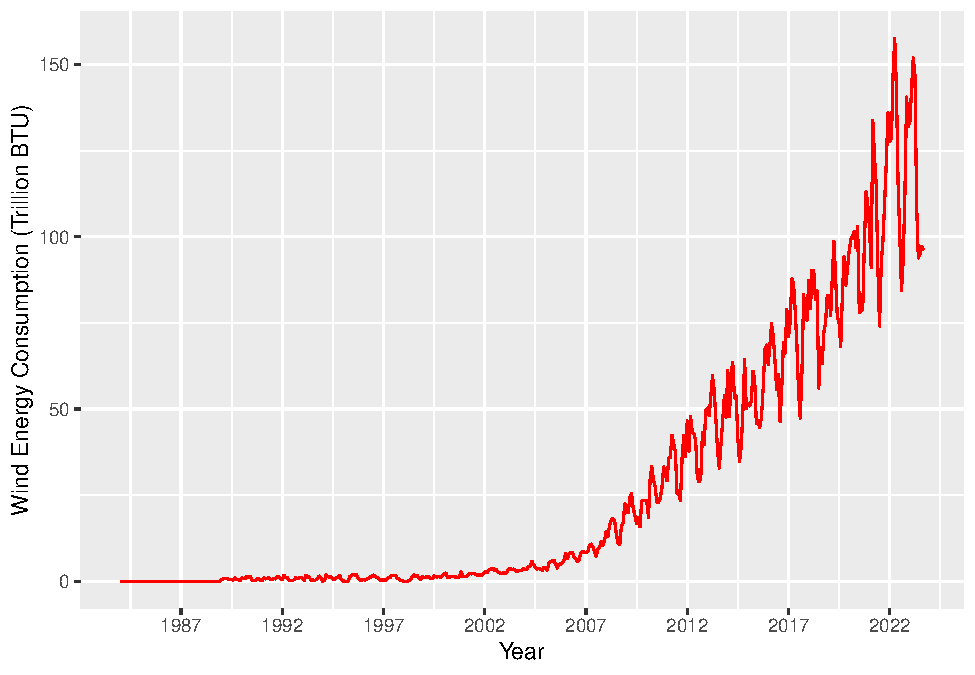
\includegraphics{JuliaKagiliery_TSA_A02_Sp24_files/figure-latex/unnamed-chunk-7-1.pdf}

\hypertarget{question-5}{%
\subsection{Question 5}\label{question-5}}

Compute the correlation between these three series. Are they
significantly correlated? Explain your answer.

\begin{Shaded}
\begin{Highlighting}[]
\NormalTok{tsenergy }\SpecialCharTok{|\textgreater{}}
  \FunctionTok{cor}\NormalTok{() }\SpecialCharTok{|\textgreater{}}
  \FunctionTok{print}\NormalTok{()}
\end{Highlighting}
\end{Shaded}

\begin{verbatim}
##                                   Total Biomass Energy Production
## Total Biomass Energy Production                        1.00000000
## Total Renewable Energy Production                      0.97074621
## Hydroelectric Power Consumption                       -0.09656318
##                                   Total Renewable Energy Production
## Total Biomass Energy Production                         0.970746212
## Total Renewable Energy Production                       1.000000000
## Hydroelectric Power Consumption                        -0.001768629
##                                   Hydroelectric Power Consumption
## Total Biomass Energy Production                      -0.096563177
## Total Renewable Energy Production                    -0.001768629
## Hydroelectric Power Consumption                       1.000000000
\end{verbatim}

It appears as though total biomass energy production and total renewable
energy production are strongly positively corelated as they have a
correlation coefficient of 0.97075. However, these two are not
correlated to hydroelectric power consumption as those coefficents are
(in magnitude) lower than 0.7 (about where I would draw the line at
taking strong conclusions about correlation).

\hypertarget{question-6}{%
\subsection{Question 6}\label{question-6}}

Compute the autocorrelation function from lag 1 up to lag 40 for these
three variables. What can you say about these plots? Do the three of
them have the same behavior?

\begin{Shaded}
\begin{Highlighting}[]
\NormalTok{tsenergy\_biomass }\OtherTok{\textless{}{-}}\NormalTok{ tsenergy[,}\DecValTok{1}\NormalTok{] }\SpecialCharTok{|\textgreater{}}
  \FunctionTok{Acf}\NormalTok{(}\AttributeTok{lag.max =} \DecValTok{40}\NormalTok{)}
\end{Highlighting}
\end{Shaded}

\includegraphics{JuliaKagiliery_TSA_A02_Sp24_files/figure-latex/unnamed-chunk-9-1.pdf}

\begin{Shaded}
\begin{Highlighting}[]
\NormalTok{tsenergy\_renewable }\OtherTok{\textless{}{-}}\NormalTok{ tsenergy[,}\DecValTok{2}\NormalTok{] }\SpecialCharTok{|\textgreater{}}
  \FunctionTok{Acf}\NormalTok{(}\AttributeTok{lag.max =} \DecValTok{40}\NormalTok{)}
\end{Highlighting}
\end{Shaded}

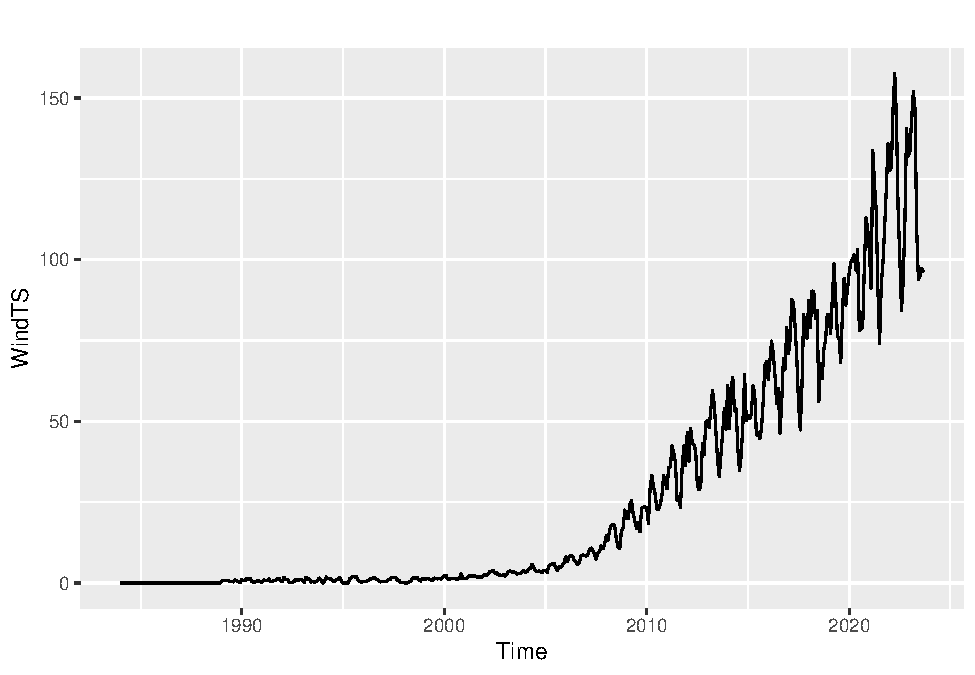
\includegraphics{JuliaKagiliery_TSA_A02_Sp24_files/figure-latex/unnamed-chunk-10-1.pdf}

\begin{Shaded}
\begin{Highlighting}[]
\NormalTok{tsenergy\_hydro }\OtherTok{\textless{}{-}}\NormalTok{ tsenergy[,}\DecValTok{3}\NormalTok{] }\SpecialCharTok{|\textgreater{}}
  \FunctionTok{Acf}\NormalTok{(}\AttributeTok{lag.max =} \DecValTok{40}\NormalTok{)}
\end{Highlighting}
\end{Shaded}

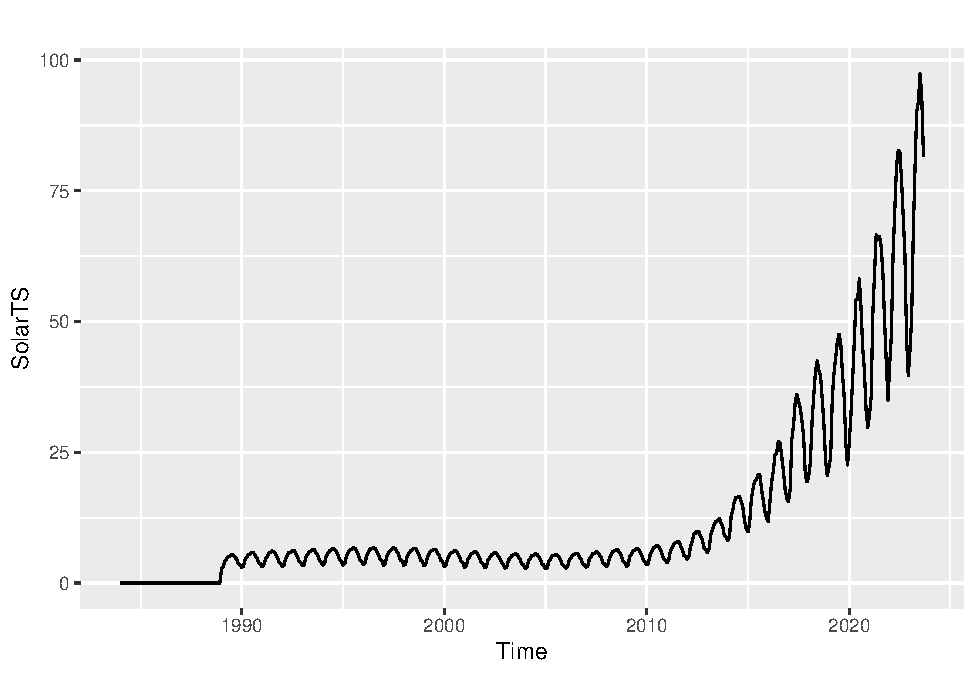
\includegraphics{JuliaKagiliery_TSA_A02_Sp24_files/figure-latex/unnamed-chunk-11-1.pdf}

\hypertarget{question-7}{%
\subsection{Question 7}\label{question-7}}

Compute the partial autocorrelation function from lag 1 to lag 40 for
these three variables. How these plots differ from the ones in Q6?

\end{document}
